\chapter{Development of the chosen solutions}

Once we have defined what we want to do in the previous chapter, \textbf{Methodology, Considerations, and Decisions on Alternative Solutions}, it is time to get to work.

\section{Graphic interface}

About user friendly graphic interface..................................

This tools can be differenciated in two very important groups, taht also will be two diferent windows of the program: REVIOSARRRRRRRRRRRRRRRRRRRRRRRR

\begin{itemize}
	\item \textbf{Analysis Window} that will recieve sound from external input, and sound that comes from System (Input form System).
	\item \textbf{DSP Window} that will recieve sound form external input, data about how it have to process, and send processed signal to Output (Output to System)
\end{itemize}

........................................................

\section{Signal Path}

Sounddevice library \cite{sounddevice}

------------------------- Arquitectura general programa general


\begin{figure}[H]
	\begin{center}
		\vspace{-2mm}
		\tikzsetnextfilename{general_path}
		\begin{tikzpicture}[node distance=30mm,on grid,auto, scale=1, bend angle=45]
			
			every node/.style={font=\small};
			
			\node (q_ext) {External Input};
			\node (null_ext) [right=of q_ext] {};
			\node (q_ana) [draw, rectangle, minimum size=1cm, below right=of null_ext]{Analysis Window};
			\node (q_dsp) [draw, rectangle, minimum size=1cm, above right=of null_ext]{DSP Window};
			\node (q_out) [right=of q_dsp, xshift=2cm]{Output to System};
			\node (q_inp) [right=of q_ana, xshift=2cm]{Input form System};
			
			
			%\node (q_delay) [draw, rectangle, minimum size=1cm, right=of null_init] {Delay Buffer};
			%\node (q_ext) [draw, rectangle, minimum size=1cm, above right=of q_delay, xshift=2cm] {Filtering and RMS Calculation of External Input};
			%\node (q_in_sys) [draw, rectangle, minimum size=1cm, below right=of q_delay, xshift=2cm] {Filtering and RMS Calculation of Input from System};
			%\node (q_diff) [draw, rectangle, minimum size=1cm, right=of q_delay, xshift=4cm] {Difference calculation};	
			
			\draw[blue, very thick, ->] (q_ext) edge node {} (q_ana);
			\draw[blue, very thick, ->] (q_ext) edge node {} (q_dsp);
			\draw[blue, very thick, ->] (q_dsp) edge node {} (q_out);
			\draw[blue, very thick, ->] (q_inp) edge node {} (q_ana);
			\draw[green, dotted, very thick, ->] (q_ana) edge [bend right=10] node {Data} (q_dsp);
			%\draw[blue, dotted, very thick, ->] (q_delay) edge[bend right=10] node {1 channel} (q_ext);
			%\draw[blue, dotted, very thick, ->] (q_delay) edge[bend right=10] node {1 channel} (q_in_sys);
			%\draw[green, very thick, ->] (q_ext) edge[bend right=10] node {Analysis Data} (q_diff);
			%\draw[green, very thick, ->] (q_in_sys) edge[bend right=10] node {Analysis Data} (q_diff);
			
		\end{tikzpicture}
		\vspace{-2mm}
	\end{center}
	\caption{General signal path}
\end{figure}

\section{Settings page [DONE]}

In order to be flexible with hardware, we need a settings window where we can tell the program which sound card, which channel, and which parameters we want to use. These parameters will also affect the resolution and fidelity of the analysis and processing, according to the sound card’s capabilities.

I will splitt setting window in tow pages:
 \begin{itemize}
 	\item \textbf{Device Settings:} Where we can define which sound card and which channels we want to use.
 	\item \textbf{Audio Settings:} Where we can define which audio parameters we want to use.
 \end{itemize}

\subsection{Device Settings}

I will use sounddevice methods to identify which sound cards and channels are available, and filter them into inputs and outputs. Then, using a questionnaire-style interface, I will let the user select which sound card and which channel they want for each required signal using a dropdown menu.

At the bottom of the page, there will be a "Confirm" button that performs some basic checks, such as verifying that the "external input" and the "input from system" are not the same input channel. Then, it will display a green message if the settings are applied successfully, or a red one if something goes wrong. Finally, it will update the values and labels on the root window to indicate which channels are currently selected.

\begin{figure}[H]
	\centering
	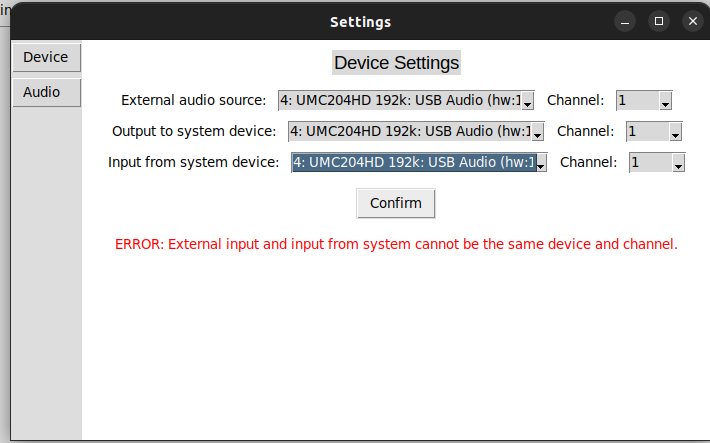
\includegraphics[width=0.8
	\linewidth]{Figures/DevSet.png}
	\caption{Device Settings page showing a red message because the user selected an invalid configuration.}
	\label{fig:Device Settings}
\end{figure}

\subsection{Audio Settings}

On this page, just like in the previous one, I will use a questionnaire-style interface with dropdown menus to define the Sample Rate, Bit Depth, and Block Size to be used.

For the Sample Rate and Bit Depth, I will suggest the most common values — such as 44,100 Hz, 48,000 Hz, 96,000 Hz, and 192,000 Hz for the sample rate, and 16, 24, and 32 bits for bit depth. However, the user is free to enter any value. The same applies to the Block Size.

At the bottom of the page, there is also a "Confirm" button, similar to the one in the "Device Settings" page. It performs basic checks, updates the selected values, and displays a message: green if everything is OK, orange in case of a warning (it applies the changes but alerts the user when a non-recommended or uncommon value is entered), and red if the Block Size is not a power of two — something required for the algorithms to work properly.

\begin{figure}[H]
	\centering
	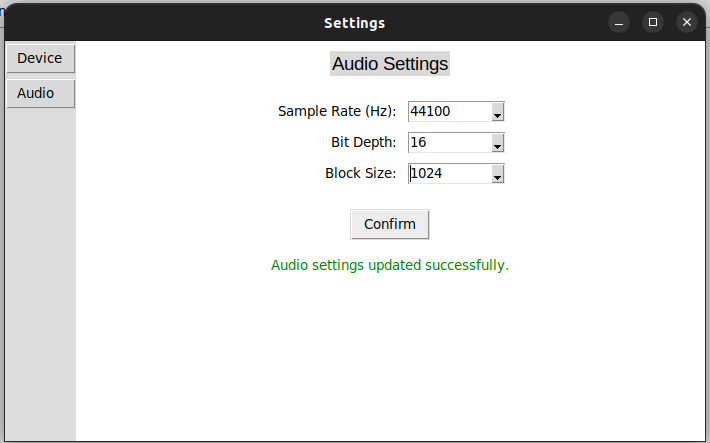
\includegraphics[width=0.8
	\linewidth]{Figures/AudSet.png}
	\caption{Audio Settings page showing a green message.}
	\label{fig:Audio Settings}
\end{figure}



\section{Acoustics analysis}

The acoustic analysis is devoloped with python librari LIBROSA\cite{librosa}

\subsection{Spectrogram (FT)}

How implemented the spectogram

\subsection{RTA [DONE]}

Usually, any form of analysis that is performed in real time can be considered \textbf{RTA} (\textit{Real-Time Analysis}). This includes a wide range of operations such as spectrum monitoring, transfer function measurements, phase and coherence analysis, and more—all happening as the signal flows. However, in my experience, in common usage, when someone refers to "RTA", they are often specifically referring to the classic 31-band graphical spectrum display. Also, the data collected on this page is especially important because it will be used to set the correction parameters. For all of that, this page has been named \textbf{RTA}.

Also, there is another conflict. When someone defines the 31 bands and their bandwidth, it is common to use the definition provided in \textbf{IEC 61260}. However, this standard does not mathematically respect the logarithmic spacing between bands. The 31 bands are defined as 1/3 of an octave per band.

\begin{table}[H]
\centering
\caption{Center frequencies for true 1/3 octave bands and IEC 61260 bands} 

	\scalebox{0.53}{
		\begin{tabular}{|c|c|c|c|c|c|c|c|c|c|c|c|}
			\hline
			1/3 octave & 19.69 & 24.8 & 31.25 & 39.37 & 49.61 & 62.5 & 78.75 & 99.21 & 125 & 157.49 & \\ \hline
			IEC 61260 & 20 & 25 & 31.5 & 40 & 50 & 63 & 80 & 100 & 125 & 160 & \\ \hline
			 & & & & & & & & & & & \\ \hline
			1/3 octave & 198,43 & 250 & 314.98 & 396.85 & 500 & 629.96 & 793.7 & 1000 & 1259.92 & 1587.4 & \\ \hline
			IEC 61260 & 200 & 250 & 315 & 400 & 500 & 630 & 800 & 1000 & 1250 & 1600 & \\ \hline
			 & & & & & & & & & & & \\ \hline
			1/3 octave & 2000 & 2519.84 & 3174.8 & 4000 & 5039.68 & 6349.6 & 8000 & 10079.37 & 12699.21 & 16000 & 20158.74 \\ \hline
			IEC 61260 & 2000 & 2500 & 3150 & 4000 & 5000 & 6300 & 8000 & 10000 & 12500 & 16000 & 20000 \\ \hline
				
		\end{tabular}
	}
\end{table}

\begin{minted}[label=\texttt{ipython}]{python3}
	"""
	In order to obtain the true 1/3 octave values, the following line of code was used with IPython3.
	The results were rounded to the second decimal place.
	"""
	
	[round(1000*2**(band/3), 2) for band in range (-17,14)]
	
\end{minted}

On the other hand, this standard is widely used in many professional devices and software. One important example is the DBX 231s graphic equalizer, which is commonly used in analog processing chains.

\begin{figure}[H]
	\centering
	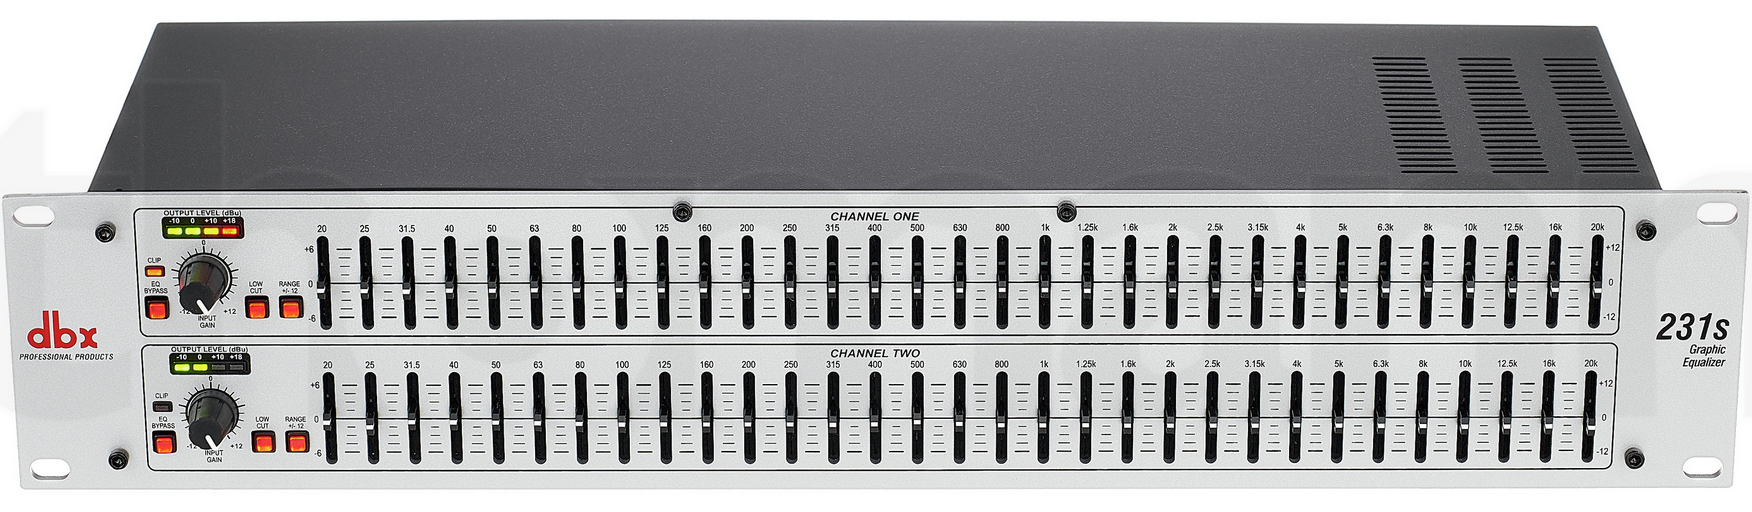
\includegraphics[width=1
	\linewidth]{Figures/DBX_231s.png}
	\caption{Image of the front panel of the DBX 231s \cite{DBX_31s}, where we can observe that the center frequency bands are the same as those defined in IEC 61260.}
	\label{fig:DBX_31s}
\end{figure}

In order to achieve the greatest possible compatibility and coherence with industry standards, I prefer to use the IEC 61260 standard.


The signal path on this page is very similar to the one used on the "FT" page. We have a buffer with two blocks of input data ("Input from external device" and "Input from system").

First, we copy the buffer data to the "delay buffer", where, if needed, the data will be adjusted to make it coincide with the applied delay. If necessary, the adjustment will use data from previous blocks stored in the same "delay buffer".

I created this buffer with the capacity to store 1 second of data, which can be used to apply a maximum delay of (1 - "Block Size in seconds") seconds.

Once the data in the "delay buffer" is adjusted, we can start applying algorithms to perform the analysis.

The algorithm is based on the calculation of RMS (\textit{root mean square}) to obtain the energy for each frequency band, which is divided using filters for each band.


\begin{figure}[H]
	\begin{center}
		\vspace{-2mm}
		\tikzsetnextfilename{RTA_page_schem}
		\begin{tikzpicture}[node distance=30mm,on grid,auto, scale=1, bend angle=45]
			
			every node/.style={font=\small};
			
			\node (q_init) [draw, rectangle, minimum size=1cm,] {Input Buffer};
			\node (null_init) [right=of q_init] {};
			\node (q_delay) [draw, rectangle, minimum size=1cm, right=of null_init] {Delay Buffer};
			\node (q_ext) [draw, rectangle, minimum size=1cm, above right=of q_delay, xshift=2cm] {Filtering and RMS Calculation of External Input};
			\node (q_in_sys) [draw, rectangle, minimum size=1cm, below right=of q_delay, xshift=2cm] {Filtering and RMS Calculation of Input from System};
			\node (q_diff) [draw, rectangle, minimum size=1cm, right=of q_delay, xshift=4cm] {Difference calculation};	
			
			\draw[blue, very thick, ->] (q_init) edge node {2 channels} (q_delay);
			\draw[blue, dotted, very thick, ->] (q_delay) edge[bend right=10] node {1 channel} (q_ext);
			\draw[blue, dotted, very thick, ->] (q_delay) edge[bend right=10] node {1 channel} (q_in_sys);
			\draw[green, very thick, ->] (q_ext) edge[bend right=10] node {Analysis Data} (q_diff);
			\draw[green, very thick, ->] (q_in_sys) edge[bend right=10] node {Analysis Data} (q_diff);
			
		\end{tikzpicture}
		\vspace{-2mm}
	\end{center}
	\caption{Diagram of the architecture of the RTA page}
\end{figure}


In this case, I'm not using any kind of windowing. As a starting point, I'm using 4th-order IIR (\textit{infinite impulse response}) Butterworth band-pass filters for each band. All these filters are created using the \texttt{scipy.signal} library \cite{scipy_signal}, which returns SOS (\textit{Second-Order Section}) parameters.

\begin{figure}[H]
	\centering
	\caption{Second-Order Sections for IIR filters with their parameters}
	\[
	H(z) = \frac{b_0 + b_1 z^{-1} + b_2 z^{-2}}{1 + a_1 z^{-1} + a_2 z^{-2}}
	\]
\end{figure}

When the program applies each filter to the signal block, it also calculates the RMS and converts it to a logarithmic scale, which will be plotted on the graph and used to calculate the difference graph.

\begin{figure}[H]
	\centering
	\caption{Root Mean Square to calculate energy from filtered signal}
	\[
	RMS = \sqrt{ \frac{1}{N} \sum_{n=0}^{N-1} x^2[n] }
	\]
\end{figure}

At the end, there is: a pause button, which blocks the update function and can be used to pause the graphics; a save button, to store the current values of the difference graph for later use in the correction window; and a time averaging section that works exactly the same as the averaging section from the FT page, except that it does not include frequency averaging (since it doesn't make sense to apply frequency averaging between bands).

\begin{figure}[H]
	\centering
	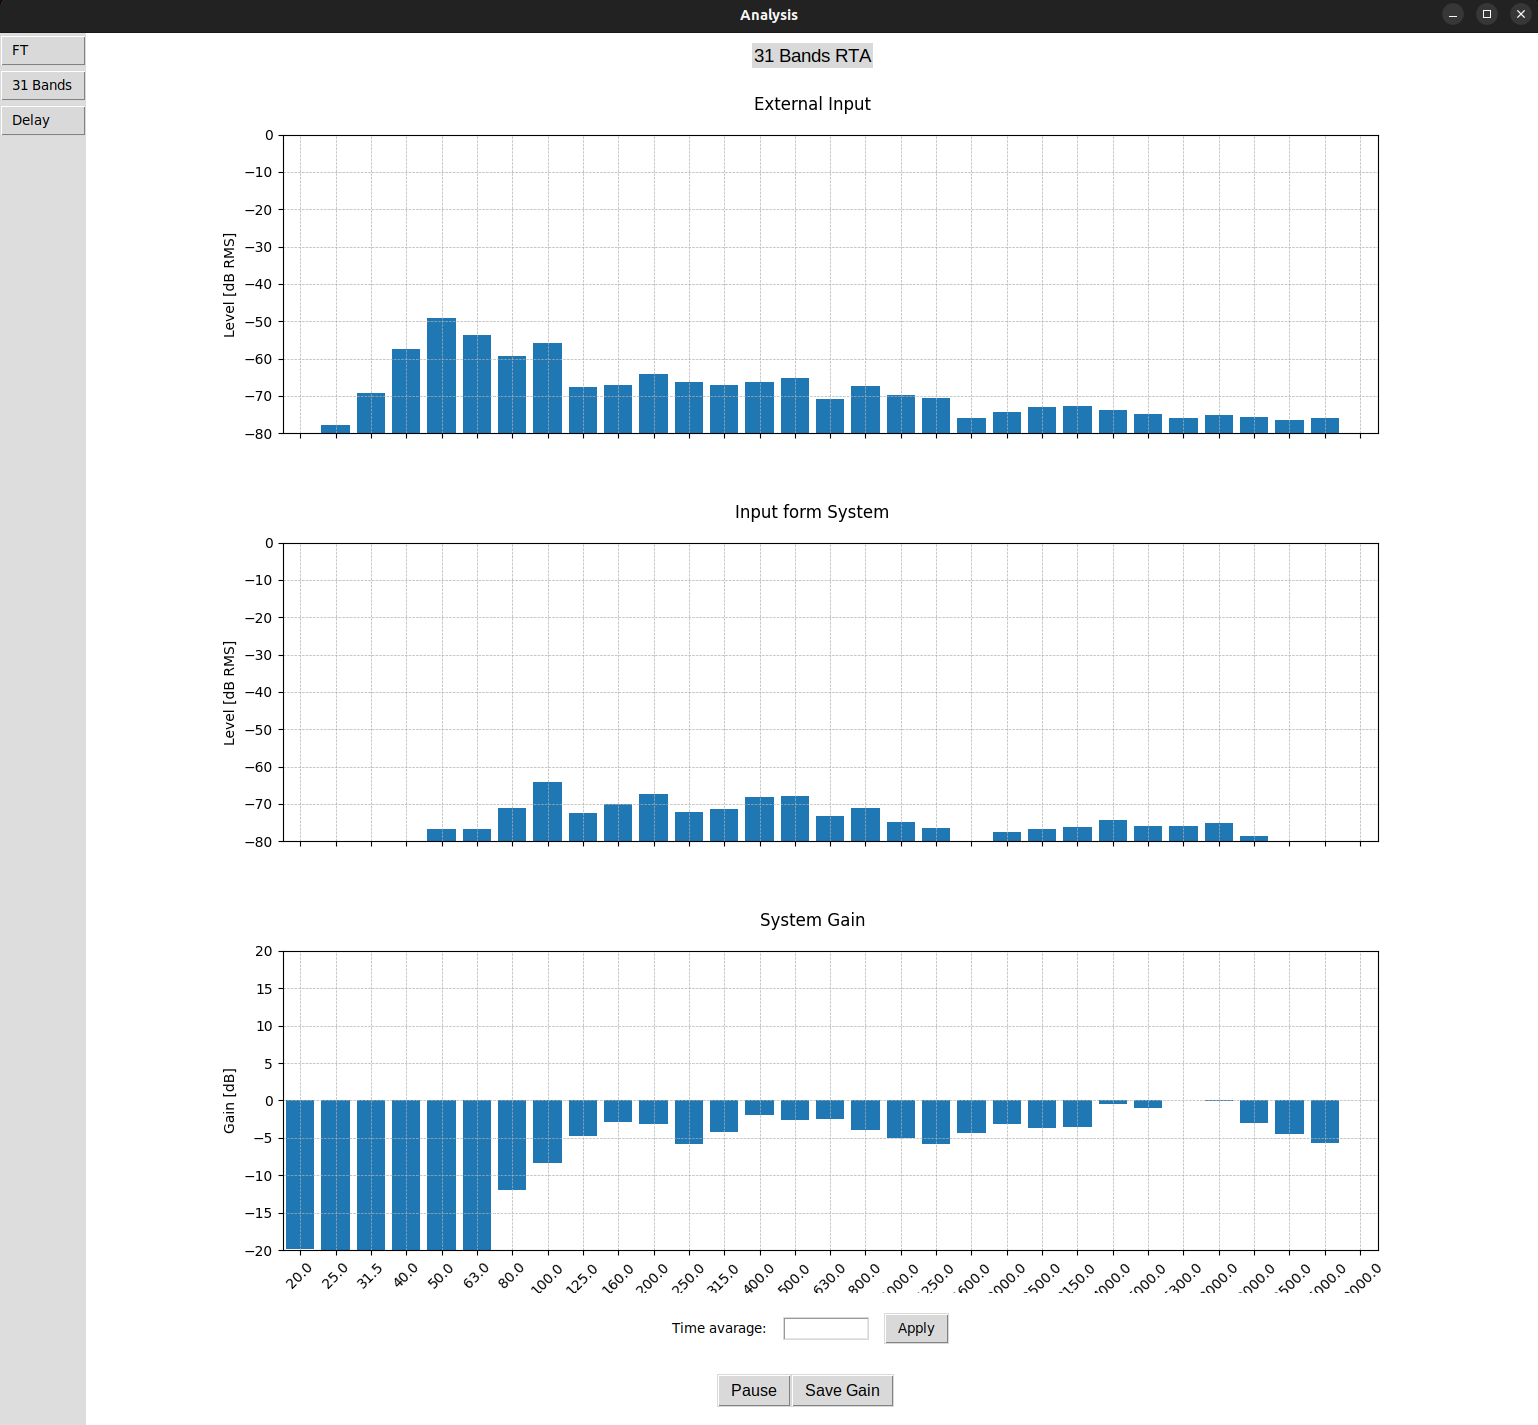
\includegraphics[width=1
	\linewidth]{Figures/RTA_page.png}
	\caption{Analysis window - RTA page.}
	\label{fig:DBX_31s}
\end{figure}


\subsection{Delay}

Explain delay page

\section{Acoustic correction}

Acoustic correction = DSP, allways have to be somethuing on the output buffer, by default, zeros.

\subsection{Bypass}

How Bypass works, and why it works bad.

\subsection{31 Bars}

Implementation of correction

\section{Integration of monitoring mechanism}

Home page and information that it appears / start, stop streams buttons...

\section{Others}

More problems that I didn't expect, losing time solving them or at least trying to. No more time to implement additional functionalities...